\section{System Design}
\label{design}
Here we cover the design of our system architecture.
We first state the overall scope we used to work toward our design goals of accuracy, transparency, scalability, and efficiency.
We then describe the main components of our system--namely, the client and broker
programs, followed by the communication protocol that these entities use.
In these sections we will highlight specific design decisions that we needed to address
in order to achieve our stated goals,
and explain how we handled them.

\subsection{Scope}
Before we could begin designing a distributed file hosting architecture,
it was necessary to define the scope for our work.
Our assumptions for this work are as follows:
\begin{itemize}
    \item \emph{Connection reliability:} The individual components of our system
    connect via TCP stream sockets in order to pass messages and data.
    This precludes reliable transmission of data, with failure detection
    and subsequent retransmission. While TCP handshakes will increase
    the latency of message passing, reliable transmission allows
    us to focus on the accuracy of our system.
    \item \emph{Conflict resolution:} Automated synchronization necessarily implies
    instances of conflicts between closely committed updates.
    Previous work (\cite{shakib1998system,hurley2004collaborative}) has been done on conflict resolution strategies in distributed domains,
    generating several viable solutions.
    We rely on these promising schemes in place of proposing our own solution,
    which is beyond the scope of this work.
    \item \emph{Security:} Our work falls in the domain
    of networked applications, and therefore is subject
    to a litany of network security attacks.
    The security community has addressed such threats
    in a body of literature that is too vast to properly reference.
    Instead we indicate where we leverage secure hashing algorithms (SHA)
    and public key infrastructure (PKI) to facilitate
    the integrity and privacy of our system,
    and leave the rest to the capable hands of security researchers.
    \end{itemize}

Having declared the scope of our project,
we now detail the D-Sync architecture.
The main components of this system are clients and brokers,
networked via TCP stream sockets.
In the following sections we will describe the primary
components and actions of each entity,
as well as any design decisions made along the way.

\subsection{Major Design Decisions}
The first design decision that we needed to cover was the synchronization
model.
We had a number of options, but to best ensure
that our system maintained data consistency
we chose Read Once Write All (ROWA). In this model,
updates are pushed to all clients in the working group
at once.
When a client needs to pull data,
the system merely fetches it from the nearest client.

In addition to selecting a synchronization model,
we also needed to specify a communication model for our system.
We chose an asynchronous communication model,
allowing users to collaborate without blocking on updates.


With the major design decisions covered, we next turn to 
the client and broker programs.

\subsection{Client}
The client program is essentially a thin local program
for handling changes to a user's local workspace.
On the one hand, it must watch the client's workspace
and detect changes to files and folders.
In order to detect changes,
the client must maintain local storage tracking
the current status of the workspace.

One of the first design decisions we had to handle on the client-side
is the discovery phase: how does a client connect to the rest of the 
D-Sync architecture?
We note that given that working groups who would potentially
use this system have inherent privacy concerns,
it is reasonable to assume that they would have interest in a secure system.
Therefore, users must be invited to the working group and the system in general.
An invited user could obtain connection information for a specific broker
to which he/she can initially connect.
Such offline information would also include any public keys needed
to verify the broker, and any symmetric keys needed for encrypting data.

Once a client has access to the network,
it can begin to collaborate with the working group.
In the next sections, we cover the various actions
that a client performs.

\subsubsection{Initialization}
In order to implement our ROWA synchronization model,
we had to take a unique approach to initializing a client.
When a client comes online,
it immediately needs to check whether its offline changes
are ahead of the system and push those changes.
After this push, the system should make the client
pull down any changes that it is behind on.
We call this initial phase the \textbf{batch update}.
This action enables our system to maintain data consistency
for online clients, which we demonstrate in our evaluation
Section~\ref{evaluation.accuracy}.

\subsubsection{Other Client Actions}
The remaining actions of the client are fairly trivial.
When the client detects an update to the local workspace,
it sends the system a request (RQST) message containing a hash
of the filename and the file's revision number.
The client then waits asynchronously for an acknowledgement
(ACK) from the broker.
We cover the need for a request message when we discuss the broker
in section \ref{broker}.
Upon receiving an ACK, the client updates the revision
number of the changed file,
and pushes that file to the system.

The only other required actions of the client are to handle
pushes coming from the broker.
If the broker pushes down a change,
the client should accept that change and update both its
local workspace and the associated file's revision number.
The client should not have to worry about calculating
revision numbers itself--that logic is handled on the broker-side.

We next turn to the broker,
the primary component of our system.
As with the client, we describe the broker's primary
function and actions.

\subsection{Broker}
\label{broker}
The broker is the computation-heavy component of our system architecture.
It is responsible for marshalling data between clients in a given
working group. The broker must handle the update requests
of all connected clients in such a way that
synchronization remains transparent to the user.
Furthermore, while all data flows through the broker,
the broker itself remains blind to the raw data itself by virtue
of hash functions or crytography on the client side.
Therefore, while the broker must maintain local storage
itself to determine the whether client requests are fresh,
this local storage need not be more than a dictionary of 
encrypted filenames mapped to revision numbers.

\subsubsection{Broker Actions}
The first action that a broker must handle is
receiving a batch update from a newly initialized client.
The broker must check whether each pushed update
is ahead of or behind the system.
Changes ahead of the system are pushed to the remaining clients.
Otherwise, the broker pulls current changes down to the initializing client.

A broker must also handle the client's normal requests,
though this is done in a similar fashion.
If the requested change is ahead of the system,
the broker pushes that change to all clients,
otherwise it pulls down a change to the requesting client.

\begin{figure}[h]
    \centering
    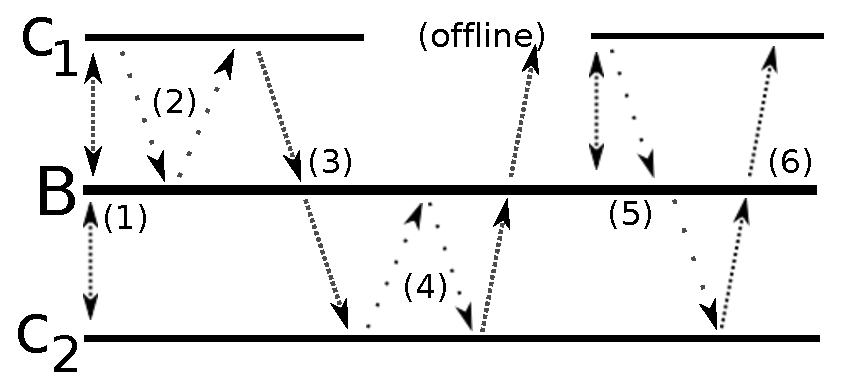
\includegraphics[scale=0.5]{figs/timeline.eps}
    \label{timeline}
    \caption{\textbf{A typical timeline involving two clients $C_1,C_2$ and broker $B$.}}
\end{figure}

Having described both the client and the broker,
we now cover a typical timeline of events
occurring between two clients, $C_1,C_2$, and broker $B$
as pictured in figure~\ref{timeline}.
In (1), both clients connect to the broker or are already connected
at this point in time. $C_1$ sends a request to the broker in (2),
which is acknowledged. $C_1$ sends out the actual change in (3),
which the broker pushes to $C_2$.
Around (4), $C_1$ goes offline and $C_2$ makes a request,
is Acknowledged, and pushes a change. This change
does not reach $C_1$, who is offline.
When $C_1$ returns in (5), $C_1$ pushes its local
workspace.  The broker determines that $C_1$ is behind
the system due to the change in (4), pulls that change
from $C_2$, and in (6) updates $C_1$.

\subsubsection{Distributed Broker}
\label{design.distributed}
While the broker description above suggests a single broker or broker network,
the broker functionality could easily be applied to a distributed manner.
In such a architecture, each client would have its own broker program.
Brokers would maintain connection information of all other connected brokers.
In the event of a channel failure or broker crash,
other brokers could try to reconnect to the disconnected broker
using exponential backoff.
In this manner, the broker network could prevent partitions of the network
due to node failures.

In addition to network partitions, a distributed broker 
solution would also have to manage requests in a new way.
When a given broker receives a request from its client,
it would contact the other brokers to determine whether the change could be committed.
Algorithms for consensus between distributed nodes would need to be leveraged
in order to make this feasible.
Once such an algorithm is put into place, however,
a client could easily connect to this new distributed broker as is.
The high level API implemented by the broker would remain the same,
with the extra consensus logic remaining transparent to the client.
We return the notion of a distributed broker in our discussion
Section~\ref{discussion}.
